\documentclass{article}

\RequirePackage{luatex85}
\usepackage{fontspec}
\usepackage[all]{xy}

\usepackage{fancyhdr}
\usepackage{extramarks}
\usepackage{amsthm,amsmath,amssymb,physics}
\usepackage{tikz}
\usepackage{float}
\usepackage{subcaption}
\usepackage{graphicx}
\usepackage{siunitx}
\usepackage{minted}
\usemintedstyle{vs}

% ====================
% Basic Document Settings
%

\usepackage{pgfplots}

\topmargin=-0.45in
\evensidemargin=0in
\oddsidemargin=0in
\textwidth=6.5in
\textheight=9.0in
\headsep=0.25in

\linespread{1.1}

\pagestyle{fancy}
\lhead{\hmwkAuthorName}
\chead{\hmwkClass : \hmwkTitle}
\rhead{\firstxmark}
\lfoot{\lastxmark}
\cfoot{\thepage}

\renewcommand\headrulewidth{0.4pt}
\renewcommand\footrulewidth{0.4pt}

\setlength\parindent{0pt}

%
% Create Problem Sections
%

\newcommand{\enterProblemHeader}[1]{
    \nobreak\extramarks{}{Problem \arabic{#1} continued on next page\ldots}\nobreak{}
    \nobreak\extramarks{Problem \arabic{#1} (continued)}{Problem \arabic{#1} continued on next page\ldots}\nobreak{}
}

\newcommand{\exitProblemHeader}[1]{
    \nobreak\extramarks{Problem \arabic{#1} (continued)}{Problem \arabic{#1} continued on next page\ldots}\nobreak{}
    \stepcounter{#1}
    \nobreak\extramarks{Problem \arabic{#1}}{}\nobreak{}
}

\setcounter{secnumdepth}{0}
\newcounter{partCounter}
\newcounter{homeworkProblemCounter}
\setcounter{homeworkProblemCounter}{1}
\nobreak\extramarks{Problem \arabic{homeworkProblemCounter}}{}\nobreak{}

%
% Homework Problem Environment
%
% This environment takes an optional argument. When given, it will adjust the
% problem counter. This is useful for when the problems given for your
% assignment aren't sequential. See the last 3 problems of this template for an
% example.
%
\newenvironment{homeworkProblem}[1][-1]{
    \ifnum#1>0
        \setcounter{homeworkProblemCounter}{#1}
    \fi

    \section{Problem \arabic{homeworkProblemCounter}}
    \setcounter{partCounter}{1}
    \enterProblemHeader{homeworkProblemCounter}
}{
    \exitProblemHeader{homeworkProblemCounter}
}


\newcommand{\hmwkTitle}{Homework\ \#5}
\newcommand{\hmwkDueDate}{20 May, 2020}
\newcommand{\hmwkClass}{CS364/AM792}
\newcommand{\hmwkAuthorName}{\textbf{Unathi K. Skosana}}

% Title Page

\title{
    \vspace{2in}
    \textmd{\textbf{\hmwkClass:\ \hmwkTitle}}\\
    \normalsize\vspace{0.1in}\small{Due\ on\ \hmwkDueDate\ at 17:00pm}\\
    \vspace{3in}
}

\author{\hmwkAuthorName}
\date{}

\renewcommand{\part}[1]{\textbf{\large Part \Alph{partCounter}}\stepcounter{partCounter}\\}

% Alias for the Solution section header
\newcommand{\solution}{\textbf{\large Solution}}

\begin{document}

\maketitle

\pagebreak

\begin{homeworkProblem}
  \textbf{(a)}
  \\
  \\

  Following the prescribed procedure to construct the matrix $X$ and its corresponding
  SVD, the singular values of $X$ are plotted below.

  \begin{figure}[H]
    \centering
    \begin{tikzpicture}
      \begin{axis}[
                  xlabel={Indices},
                  ylabel={Values},
      ]
        \addplot table[only marks, x index=0, y index=1, col
          sep=comma]{./singular_values.dat};
        \end{axis}
      \end{tikzpicture}
      \caption{Singular values of $X$}%
    \label{fig:sing_vals}
  \end{figure}

  From the plot above, it seems like $> 2000$ is a sensible threshold. This
  particular threshold gives an alpha value of $\alpha=19$. Figure
  ~\ref{fig:avg} and ~\ref{fig:eigfaces} show the average face $\mathbf{a}$ and
  the first five eigenfaces, rescaled and shifted back to grayscale.

  \begin{figure}[H]
    \centering
    \begin{subfigure}{0.4\textwidth}
      \centering
      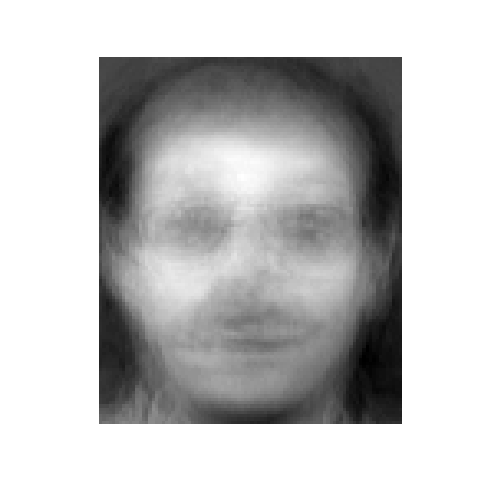
\includegraphics[width=.5\linewidth]{./images/average.png}
      \caption{Average Face}
      \label{fig:avg}
    \end{subfigure}%
    \begin{subfigure}{0.59\textwidth}
      \centering
      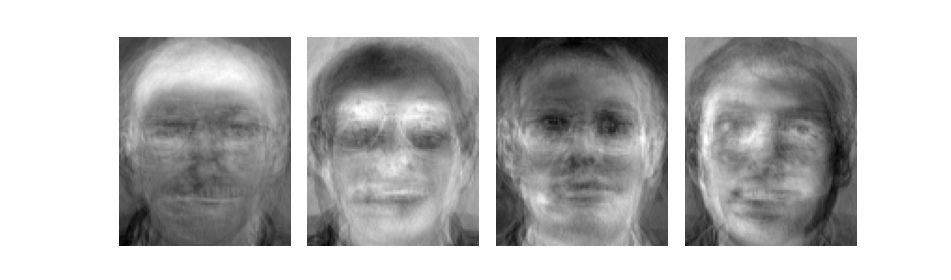
\includegraphics[width=1.0\linewidth]{./images/eigenfaces.png}
      \caption{First Five Eigenfaces}
      \label{fig:eigfaces}
    \end{subfigure}
  \end{figure}

  \textbf{(b)}
  \\
  \\

  The acquisition of $U_\alpha$ and $\mathbf{a}$ allows one to encode all the
  test images to their corresponding eigenface representations, $\mathbf{y}_i$.
  From this representation we can reconstruct a low dimension representation of
  a test image via

  \begin{align*}
    \mathbf{\hat{f}}_i = \mathbf{a} + U_\alpha \mathbf{y}_i
  \end{align*}

  \pagebreak

  Figure~\ref{fig:recon} shows a sample of a few such low dimension representations and their
  originals, the image information seems to be
  captured well enough as some of the features of the original are recognizable.

  \begin{figure}[H]
    \centering
    \begin{subfigure}{0.5\textwidth}
      \centering
      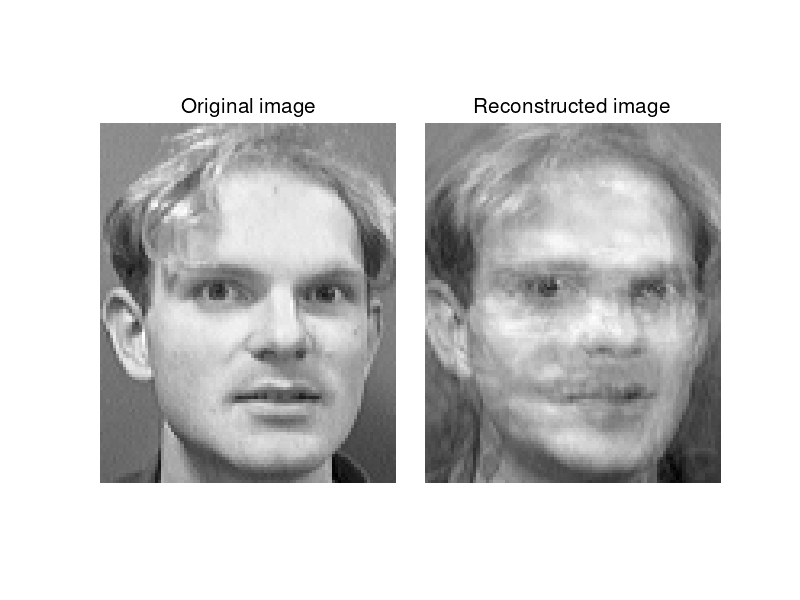
\includegraphics[width=1.\linewidth]{./images/encoded_1.png}
    \end{subfigure}%
    \begin{subfigure}{0.5\textwidth}
      \centering
      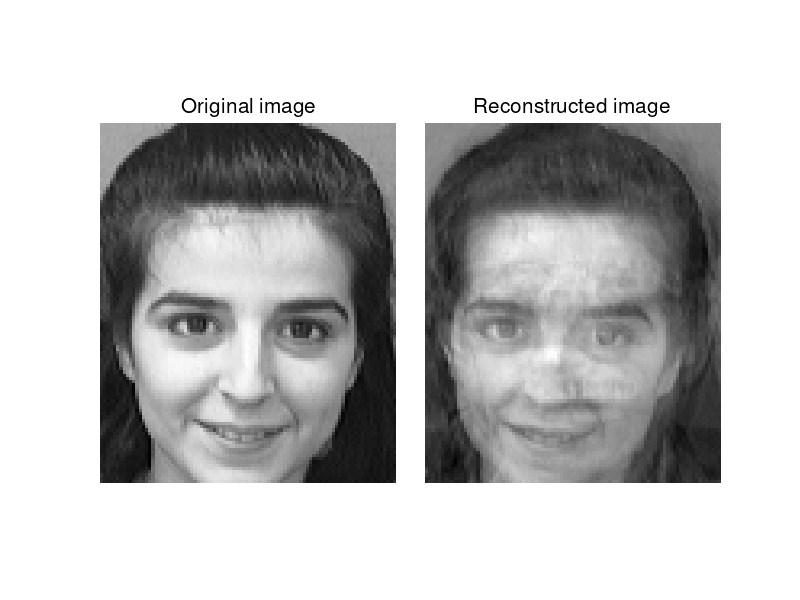
\includegraphics[width=1.\linewidth]{./images/encoded_2.png}
    \end{subfigure}
    \begin{subfigure}{0.5\textwidth}
      \centering
      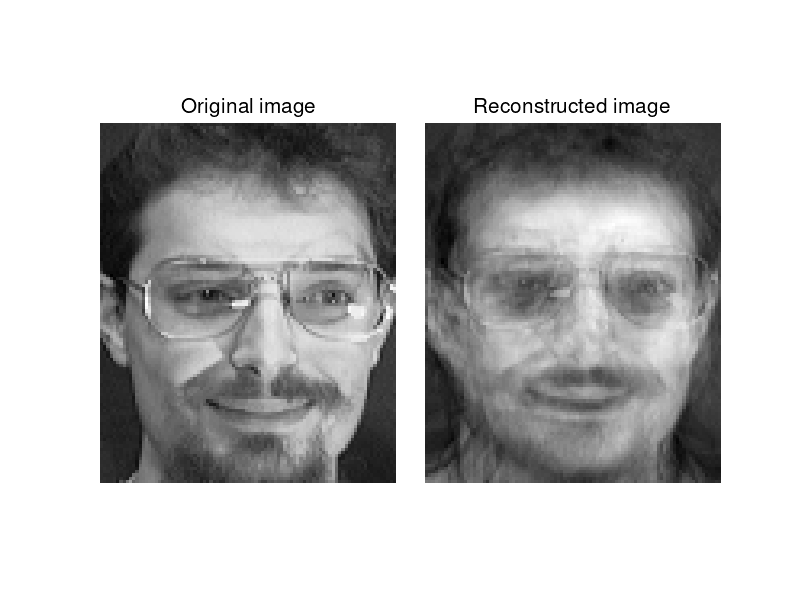
\includegraphics[width=1.\linewidth]{./images/encoded_3.png}
    \end{subfigure}%
    \begin{subfigure}{0.5\textwidth}
      \centering
      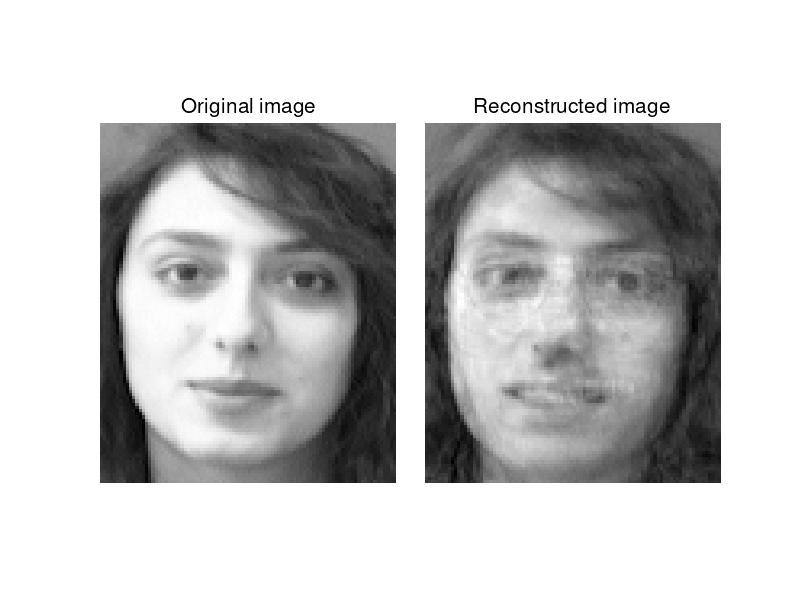
\includegraphics[width=1.\linewidth]{./images/encoded_4.png}
    \end{subfigure}
    \begin{subfigure}{0.5\textwidth}
      \centering
      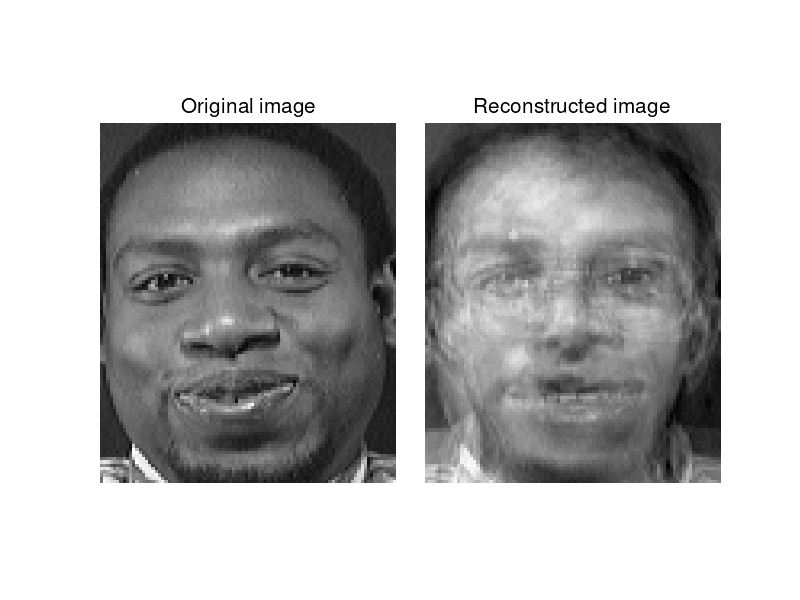
\includegraphics[width=1.\linewidth]{./images/encoded_5.png}
    \end{subfigure}%
    \begin{subfigure}{0.5\textwidth}
      \centering
      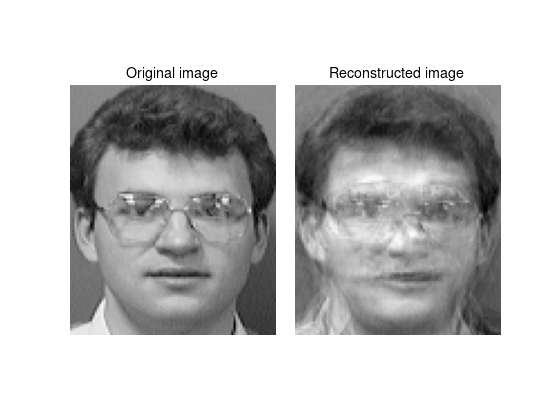
\includegraphics[width=1.\linewidth]{./images/encoded_6.png}
    \end{subfigure}
    \caption{Originals and Low Dimensions Representations Of Test Images}
    \label{fig:recon}
  \end{figure}

  \pagebreak

  \textbf{(c)}
  \\
  \\

  To accomplish classification, we first have to get the eigenface representations of the training
  and test set images, then for every image $i$ in each test set, calculate

  \begin{align*}
    d_j = \Vert \mathbf{y}_i - \mathbf{y}'_{j}\Vert
  \end{align*}

  where $\mathbf{y}'_j$ is the eigenface representation of the $j^\mathrm{th}$ image
  in the training set. \\

  The index $i^*$ of the minimum value of $\mathbf{d}$ is
  the closest neighbor of the $i^\mathrm{th}$ test image. If $i = i^*$, then the
  image was correctly matched and incorrectly matched otherwise. Below are the
  test images with their corresponding matches as described.

  \begin{figure}[H]
    \centering
    \begin{subfigure}{0.5\textwidth}
      \centering
      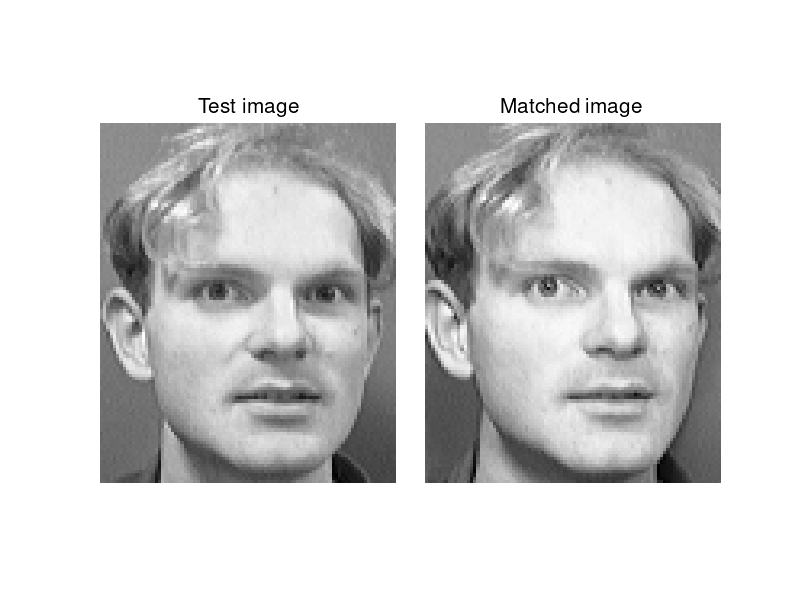
\includegraphics[width=1.\linewidth]{./images/match_1.png}
    \end{subfigure}%
    \begin{subfigure}{0.5\textwidth}
      \centering
      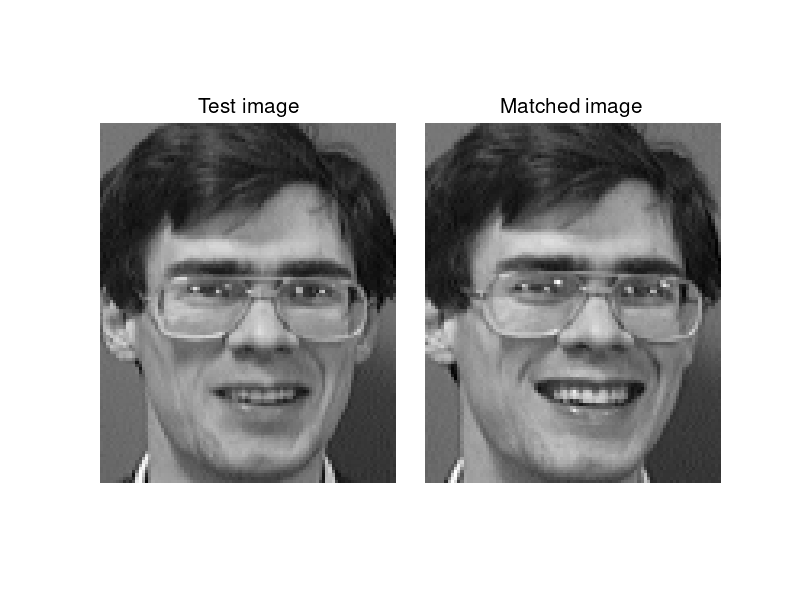
\includegraphics[width=1.\linewidth]{./images/match_2.png}
    \end{subfigure}
    \begin{subfigure}{0.5\textwidth}
      \centering
      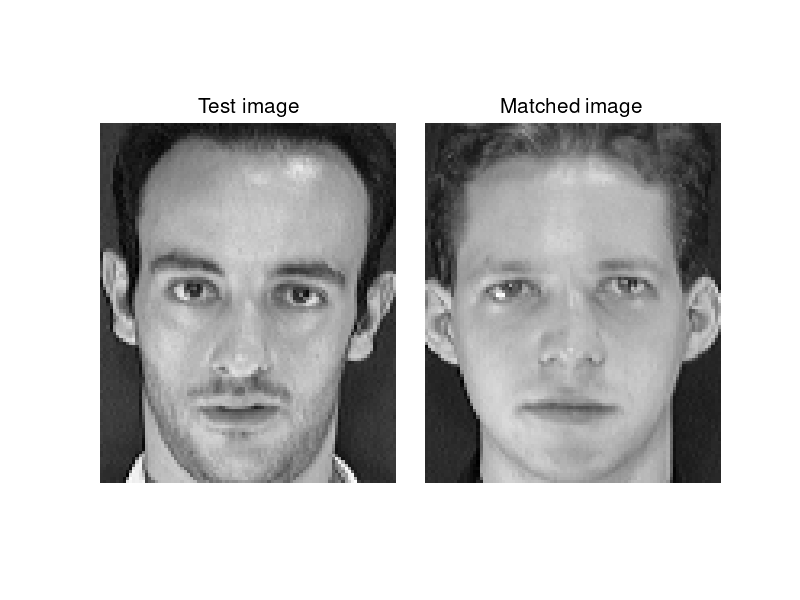
\includegraphics[width=1.\linewidth]{./images/match_3.png}
    \end{subfigure}%
    \begin{subfigure}{0.5\textwidth}
      \centering
      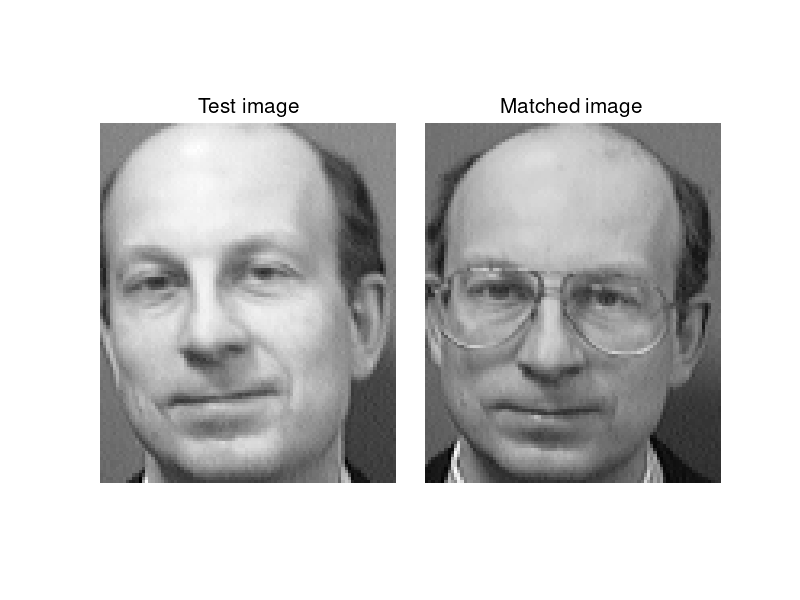
\includegraphics[width=1.\linewidth]{./images/match_4.png}
    \end{subfigure}
  \end{figure}
  \begin{figure}[H]
    \begin{subfigure}{0.5\textwidth}
      \centering
      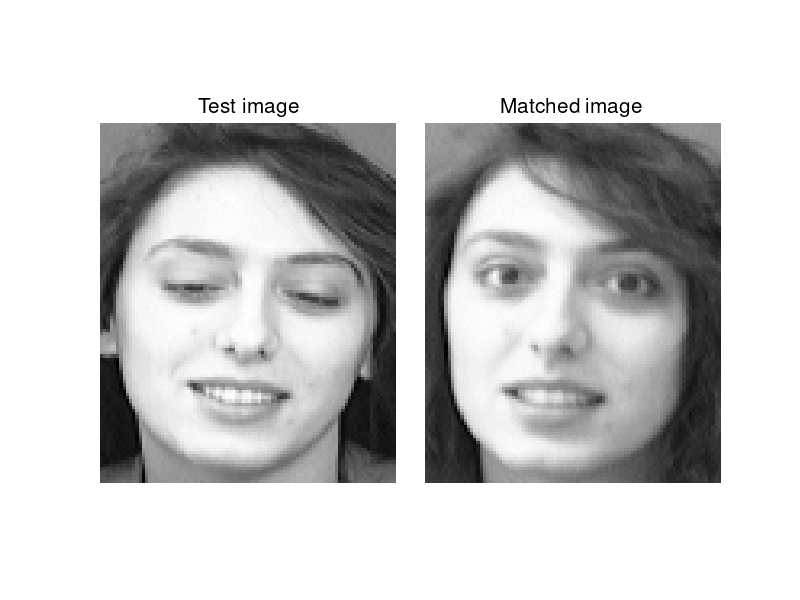
\includegraphics[width=1.\linewidth]{./images/match_5.png}
    \end{subfigure}%
    \begin{subfigure}{0.5\textwidth}
      \centering
      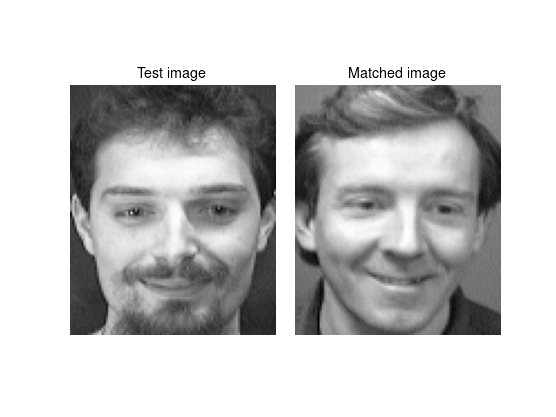
\includegraphics[width=1.\linewidth]{./images/match_6.png}
    \end{subfigure}
    \caption{Test images And Their Closest Neighbors From The Training Set}
    \label{fig:cln}
  \end{figure}

  The accuracy of the matching was roughly $78.75 \%$ and we can see some of the
  inaccuracies in the above sample.

\end{homeworkProblem}

\pagebreak

\begin{homeworkProblem}
  \textbf{(a)}
  \\
  \\

  For this question, I used the SIFT features already provided in the
  accompanying material. Reading the dataset into python, I was able to
  arbitrarily assign labels to images according to what class they belonged to,
  i.e, $\mathrm{Coast}\to0, \mathrm{Forest}\to1, \mathrm{Highway}\to2$ etc. The class
  labels were assigned this sequence of numbers in ascending alphabetic order.
  \\

  Collecting all descriptors of the training set into one giant array and
  feeding them to the \mintinline{python}{sklearn}'s \mintinline{python}{Kmeans} module for a fit 
  with $k = 60$, giving a vocabulary of $60$ words. From this vocabulary, we can run through
  image descriptors and use \mintinline{python}{kmeans.fit(descr)} to assign
  them to cluster center labels, thus the Bag Of Words representation of an
  image becomes a histogram of the cluster center labels the image's descriptors
  belong to.
  \\

  Here are a few representative samples of histograms from the first four
  classes in the training set.

\begin{figure}[H]
  \centering
  \begin{subfigure}{.4\textwidth}
    \begin{tikzpicture}[scale=0.75]
        \begin{axis}[ybar,
                    bar width=.1cm,
                    enlarge x limits=0.1,
                    ymin=0,
                    ymax=1,
                    ticks=both,
                    ytick={0, .25, 0.5, 0.75, 1.0},
                    yticklabels={0, 0.25, 0.5, 0.75, 1.0},
                    xlabel={Labels},
                    ylabel={Probabilities}
                    ]
            \addplot table[x index = {0}, y index = {1}, col
              sep=comma]{./hist_1.dat};
        \end{axis}
      \end{tikzpicture}
  \end{subfigure}%
  \begin{subfigure}{.4\textwidth}
    \begin{tikzpicture}[scale=0.75]
      \begin{axis}[ybar,
                  bar width=.1cm,
                  enlarge x limits=0.1,
                  ymin=0,
                  ymax=1,
                  ticks=both,
                  ytick={0, 0.25, 0.5, 0.75, 1.0},
                  yticklabels={0, 0.25, 0.5, 0.75, 1.0},
                  xlabel={Labels},
                  ylabel={Probabilities}
                  ]
          \addplot table[x index = {0}, y index = {1}, col
            sep=comma]{./hist_2.dat};
      \end{axis}
    \end{tikzpicture}
  \end{subfigure}

  \begin{subfigure}{.4\textwidth}
    \begin{tikzpicture}[scale=0.75]
      \begin{axis}[ybar,
                  bar width=.1cm,
                  enlarge x limits=0.1,
                  ymin=0,
                  ymax=1,
                  ticks=both,
                  ytick={0, 0.25, 0.5, 0.75, 1.0},
                  yticklabels={0, 0.25, 0.5, 0.75, 1.0},
                  xlabel={Labels},
                  ylabel={Probabilities}
                  ]
          \addplot table[x index = {0}, y index = {1}, col
            sep=comma]{./hist_3.dat};
      \end{axis}
    \end{tikzpicture}
  \end{subfigure}
  \begin{subfigure}{.4\textwidth}
    \begin{tikzpicture}[scale=0.75]
      \begin{axis}[ybar,
                  bar width=.1cm,
                  enlarge x limits=0.1,
                  ymin=0,
                  ymax=1,
                  ticks=both,
                  ytick={0, 0.25, 0.5, 0.75, 1.0},
                  yticklabels={0, 0.25, 0.5, 0.75, 1.0},
                  xlabel={Labels},
                  ylabel={Probabilities}
                  ]
          \addplot table[x index = {0}, y index = {1}, col
            sep=comma]{./hist_4.dat};
      \end{axis}
    \end{tikzpicture}
  \end{subfigure}
\end{figure}

\pagebreak

\textbf{(b)}
\\
\\

Now from the bag of words representation of the training set, we assign to it labels
according to what class each image belongs to,  as described earlier. We can fit
the training set histograms along side with their correct labels with \mintinline{python}{sklearn}'s
\mintinline{python}{svm} module, initialized with

\begin{minted}{python}
    clf = svm.SVC(C=50.0, decision_function_shape='ovo', probability=False,
                        kernel='linear', cache_size=1000)
\end{minted}{python}

where $C$ is the regularization parameter, here set to $50$ (will elaborate
later on the choice) and decision\_function\_shape specifies
the classification approach for multi-class classification, in this case it is
set to one versus one, and the kernel is specified as linear.
\\

We can fit the training data with

\\

\begin{minted}{python}
    clf.fit(flatten(train_bow_hist), flatten(train_labels))
\end{minted}{python}

where \mintinline{python}{train_bow_hist} is an array with shape

\begin{minted}{python}
  (num_classes=9, samples_in_each_class=100, number_of_vwords=60)
\end{minted}

with \mintinline{python}{train_labels} having a similar shape, containing the labels
for entries in \mintinline{python}{train_bow_hist}. The classifier can infer the number
of classes by counting only unique elements in
\mintinline{python}{flatten(train_labels))}.
\\

Finally we can use the fitted classifier to classify the test data. The below
table shows the classification report

\begin{figure}[H]
  \centering
    \begin{tabular}{c l l l l}
      class      &precision & recall & f1-score & support \\
      \hline
      0       &0.68      &0.50      &0.57       &260 \\
      1       &0.78      &0.93      &0.85       &228\\
      2       &0.51      &0.47      &0.49       &160\\
      3       &0.50      &0.51      &0.50       &110\\
      4       &0.71      &0.63      &0.67       &274\\
      5       &0.64      &0.66      &0.65       &115\\
      6       &0.70      &0.70      &0.70       &215\\
      7       &0.56      &0.61      &0.59       &192\\
      8       &0.64      &0.85      &0.73       &141\\
      \hline
    accuracy        &          &          & 0.65     &1695 \\
    macro avg       &0.64      &0.65      &0.64      &1695 \\
    weighted avg    &0.65      &0.65      &0.65      &1695
  \end{tabular}
\end{figure}

\pagebreak

Reporting an accuracy of $\sim 65 \%$. The confusion matrix for this particular
instance of the classifier is given by

\begin{align*}
  M_\mathcal{C} = \begin{bmatrix}
    129 & 15 & 44 & 2 & 31 & 2 & 3 & 26 & 8\\
    0 & 213 & 0 & 0 & 7 & 0 & 2 & 2 & 4\\
    33 & 0 & 75 & 0 & 9 & 1 & 7 & 22 & 13\\
    1 & 0 & 1 & 56 & 1 & 24 & 7 & 12 & 8\\
    26 & 30 & 12 & 0 & 172 & 0 & 6 & 14 & 14\\
    0 & 0 & 2 & 27 & 2 & 76 & 4 & 1 & 3\\
    0 & 9 & 4 & 12 & 8 & 10 & 150 & 15 & 7\\
    2 & 4 & 7 & 7 & 11 & 3 & 30 & 118 & 10\\
    0 & 1 & 3 & 8 & 2 & 2 & 4 & 1 & 120\\
  \end{bmatrix}
\end{align*}
\\

Here are few samples of incorrectly classified test images
\\

\begin{figure}[H]
  \centering
  \begin{subfigure}{0.5\textwidth}
    \caption{Coast scene incorrectly classified as a highway}
    \centering
    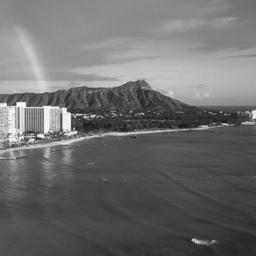
\includegraphics[width=.5\linewidth]{./images/0_high.jpg}
  \end{subfigure}%
  \begin{subfigure}{0.5\textwidth}
    \centering
    \caption{Coast scene incorrectly classified as a suburb scene}
    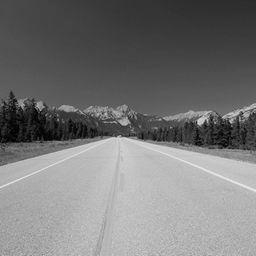
\includegraphics[width=.5\linewidth]{./images/0_surb.jpg}
  \end{subfigure}
  \begin{subfigure}{0.5\textwidth}
    \centering
    \caption{Forest scene incorrectly classified as a mountain scene}
    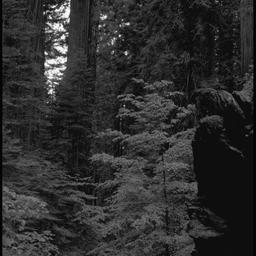
\includegraphics[width=.5\linewidth]{./images/1_mount.jpg}
  \end{subfigure}%
  \begin{subfigure}{0.5\textwidth}
    \centering
    \caption{Forest scene incorrectly classified as a street scene}
    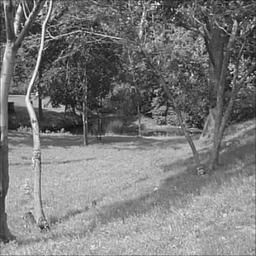
\includegraphics[width=.5\linewidth]{./images/1_street.jpg}
  \end{subfigure}
  \begin{subfigure}{0.5\textwidth}
    \centering
    \caption{Highway scene incorrectly classified as a coast scene}
    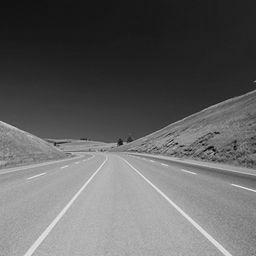
\includegraphics[width=.5\linewidth]{./images/2_coas.jpg}
  \end{subfigure}%
  \begin{subfigure}{0.5\textwidth}
    \centering
    \caption{Highway scene incorrectly classified as a office scene}
    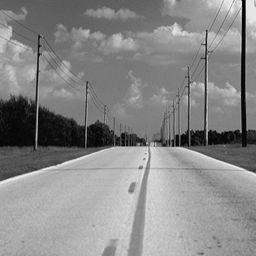
\includegraphics[width=.5\linewidth]{./images/2_offi.jpg}
  \end{subfigure}
\end{figure}

\begin{figure}[H]\ContinuedFloat
  \begin{subfigure}{0.5\textwidth}
    \centering
    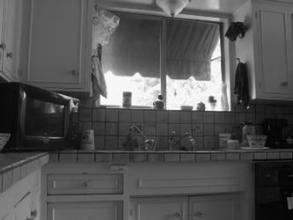
\includegraphics[width=.5\linewidth]{./images/3_offi.jpg}
    \caption{Kitchen scene incorrectly classified as a office scene}
  \end{subfigure}%
  \begin{subfigure}{0.5\textwidth}
    \centering
    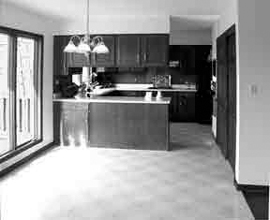
\includegraphics[width=.5\linewidth]{./images/3_surb.jpg}
    \caption{Kitchen scene incorrectly classified as a suburb scene}
  \end{subfigure}
  \begin{subfigure}{0.5\textwidth}
    \centering
    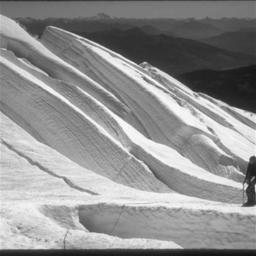
\includegraphics[width=.5\linewidth]{./images/4_coas.jpg}
    \caption{Mountain scene incorrectly classified as a coast scene}
  \end{subfigure}%
  \begin{subfigure}{0.5\textwidth}
    \centering
    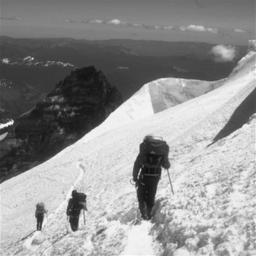
\includegraphics[width=.5\linewidth]{./images/4_surb.jpg}
    \caption{Mountain scene incorrectly classified as a suburb scene}
  \end{subfigure}
\end{figure}

\pagebreak
Here are few samples of correctly classified test images
\\


\begin{figure}[H]
  \begin{subfigure}{0.5\textwidth}
    \centering
    \caption{Office scene correctly identified}
    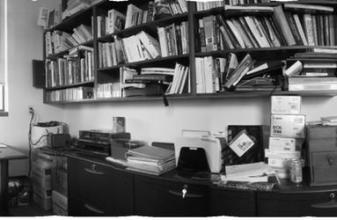
\includegraphics[width=.5\linewidth]{./images/5_off.jpg}
  \end{subfigure}%
  \begin{subfigure}{0.5\textwidth}
    \centering
    \caption{Office scene office identified}
    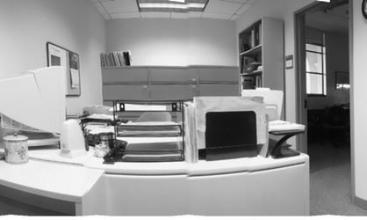
\includegraphics[width=.5\linewidth]{./images/5_ooff.jpg}
  \end{subfigure}
  \begin{subfigure}{0.5\textwidth}
    \centering
    \caption{Store scene office identified}
    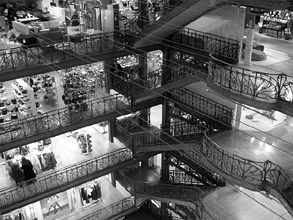
\includegraphics[width=.5\linewidth]{./images/6_stor.jpg}
  \end{subfigure}%
  \begin{subfigure}{0.5\textwidth}
    \centering
    \caption{Store scene office identified}
    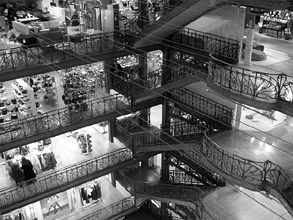
\includegraphics[width=.5\linewidth]{./images/6_stor.jpg}
  \end{subfigure}
  \begin{subfigure}{0.5\textwidth}
    \centering
    \caption{Street scene office identified}
    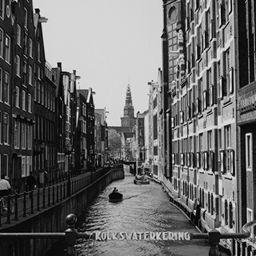
\includegraphics[width=.5\linewidth]{./images/7_street.jpg}
  \end{subfigure}%
  \begin{subfigure}{0.5\textwidth}
    \centering
    \caption{Street scene office identified}
    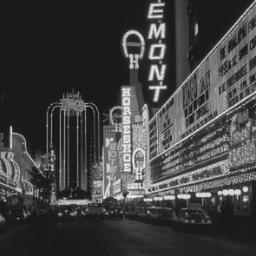
\includegraphics[width=.5\linewidth]{./images/7_sstreet.jpg}
  \end{subfigure}
  \begin{subfigure}{0.5\textwidth}
    \centering
    \caption{Suburb scene office identified}
    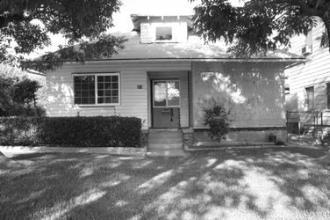
\includegraphics[width=.5\linewidth]{./images/8_ssurb.jpg}
  \end{subfigure}%
  \begin{subfigure}{0.5\textwidth}
    \centering
    \caption{Suburb scene office identified}
    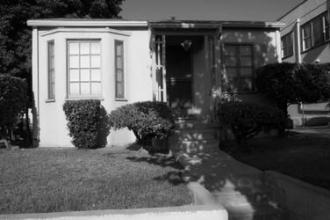
\includegraphics[width=.5\linewidth]{./images/7_surb.jpg}
  \end{subfigure}
\end{figure}

\\
\textbf{Discusion:}
\\
On $k$-means clustering, I've noted that increasing $k$ beyond $50-60$ doesn't marginally improve the
end result (test accuracy), in fact there seems to be some point slightly above $60$ where
increasing $k$ any further makes the result less accurate, thus it seems that
that a locally optimal value of $k$ lies just above $60$. Training the $36$ SVMs
for classification while having a small $ 1.0 < C \leq 5.0 $  (loose constraints
or large margin) produced inaccurate results $(36\% - 40\%)$. These results are improved when $5.0 \leq C \leq 50.00$ with
a high of $65 \%$ test accuracy, similar to the $k$-means clustering scenario,
increasing $C$ any further becomes detrimental to the test accuracy. This is
expected as this is a drawback of narrow margins fit too closely to the
training set ; the classifier does not fare well when classifying new data.

\end{homeworkProblem}

\end{document}
